\documentclass[handout]{beamer}
\mode<presentation> {%
	\usetheme[]{Boadilla}
	\usecolortheme{orchid}
	\setbeamercovered{transparent}
	\setbeamersize{text margin left=0.7cm}
  \setbeamersize{text margin right=0.7cm}
  \setbeamertemplate{enumerate item}[square]
  \setbeamertemplate{enumerate subitem}[circle]
  \setbeamertemplate{enumerate subsubitem}[>]
  \setbeamertemplate{itemize item}[square]
  \setbeamertemplate{itemize subitem}[circle]
  \setbeamertemplate{itemize subsubitem}[>]
}


\usepackage{pstricks}
\usepackage{pst-node}
\usepackage{bm}
\usepackage[utf8]{inputenc}
\usepackage[spanish]{babel}
\usepackage{times}
\usepackage[T1]{fontenc}
\usepackage{graphicx}
\usepackage{multirow}
\usepackage{pifont}
\usepackage{rotating}
\usepackage{colortbl}
\usepackage[framed]{mcode}
\usepackage{verbatim}
\usepackage{tikz}
\usetikzlibrary{positioning}
\usetikzlibrary{shapes.multipart,decorations.pathreplacing}
\tikzstyle{bloque}=[rectangle,rounded corners=2pt,draw=black!60,fill=black!5,very thick,minimum size=5mm,align=center]%
\tikzstyle{arrow}=[very thick,color=black!60]%


\definecolor{olivegreen}{rgb}{0.0,0.5,0.0}
\definecolor{general}{rgb}{0.9 0.9 1}%
\newrgbcolor{colorsistema}{0 1 1}
\newrgbcolor{colorviolet}{0.9 0.8 1}

\author[J. Chacón]{%[Author, Another] % (optional, use only with lots of authors)
\textit{Ingeniería Electrónica de Comunicaciones }\\
\vspace{0.6cm}
\small Jesús Chacón Sombría}%\inst{1} \and S.~Another\inst{2}}


\institute[DACYA. UCM] % (optional, but mostly needed)
{
  %\inst{1}%

\footnotesize  Departamento de Arquitectura de Computadores y Automática.\\
  Universidad Complutense de Madrid
  }

\date[Diseño de filtros] % (optional)
{\footnotesize Curso 2025-2026}%{\today / Master}
\subject{Talks}

\pgfdeclareimage[height=0.75cm]{logo}{ucm}

\usepackage[absolute,overlay]{textpos}
\setlength{\TPHorizModule}{1mm}
\setlength{\TPVertModule}{1mm}
\newcommand{\MyLogo}{%
\begin{textblock}{14}(116.0,0.6)
  \pgfuseimage{logo}
\end{textblock}
}

\makeatletter
\numberwithin{section}{part}
\AtBeginPart{
\beamer@tocsectionumber=0\relax
\frame{\partpage}
}
\makeatother

\begin{document}

\begin{frame}
  \titlepage
\end{frame}

\newcommand*\oldmacro{}%
\let\oldmacro\insertshorttitle%
\renewcommand*\insertshorttitle{%
 \MyLogo
  \oldmacro\hfill%
}

\AtBeginSection[]{}
\AtBeginSubsection[]{}

  

%%%%%%%%%%%%%%Empieza la presentacion%%%%%%%%%%%%%%%%%%%%%%%%%%%%%%%%%%%%

%\begin{frame}
%\frametitle{Esquema}
 %   \tableofcontents
%\end{frame}

\section{Objetivos}

\begin{frame}
\frametitle{Objetivos del tema}

\begin{itemize}
\item Aprender a utilizar técnicas  de diseño de filtros generales (paso baja, paso alta, paso banda y supresor de banda):

\begin{itemize}
\normalsize
\visible<2->{
\item Continuos: 
\begin{itemize}
\small
\item Obtener únicamente la función de transferencia del filtro (no vamos a diseñar el sistema analógico que lo representa)
\item Aproximaciones a los filtros ideales
\end{itemize}
}

\visible<3->{
\item Discretos:
\begin{itemize}
\small
\item Filtros IIR: a partir de las aproximaciones de filtros continuos
\item Filtros FIR: a partir de la transformada de Fourier con ventana
\end{itemize}

}

\end{itemize}

\visible<4->{\item Aprender a diseñar filtros específicos/a medida}

\end{itemize}

\end{frame}


\section{Introducción}

\begin{frame}\frametitle{Filtros}
    \begin{figure}
        \centering
        \small
        \begin{tikzpicture}
          \node[bloque,minimum width=15mm] (T) {H($\cdot$)};
          \node (x) [left=of T] {};
          \node (y) [right=of T] {};
          \draw[arrow,->] (x.east) -- (T.west) node [midway,above] {$x(\cdot)$};
          \draw[arrow,->] (T.east) -- (y.west) node [midway,above] {$y(\cdot)$};
        \end{tikzpicture}
    \end{figure}
    \begin{itemize}
        \item \alert{¿Qué es un filtro?}\vspace{0.1cm}
        \begin{itemize}\footnotesize
            \item<2-> Dispositivo que modifica selectivamente las frecuencias de una señal.\vspace{0.1cm}
            \item<3-> Consideramos sistemas LTI estables.\vspace{0.1cm}
            \item<4-> Caracterización mediante:
            \begin{itemize}\scriptsize
                \item<4-> Respuesta en frecuencia: \color{blue}$H(j\omega)$ \color{black} o \color{blue}$H(\textrm{e}^{j\omega})$\color{black} (continuo/discreto).\vspace{0.05cm}
                \item<4-> Respuesta impulso: \color{blue}$h(t)$ \color{black} o \color{blue}$h[n]$\color{black} (continuo/discreto).
            \end{itemize}
        \end{itemize}
    \end{itemize}
\end{frame}

\subsection{Filtros Ideales}

\begin{frame}\frametitle{Filtros Ideales}
    \begin{columns}[T]
        \begin{column}{5cm}
            \visible<1->{
                \scriptsize
                \centering{Filtro paso bajo}
                \vspace{0.1cm}
                $H(j\omega)\!=\!\left \{  \!\!\!\begin{array}{l} 1, \: \textrm{para } |\omega|\!\!<\!\!\omega_c\\0, \:\textrm{c.c.}  \end{array}\right .$
                \vspace{-0.4cm}
                \begin{figure}
                    \centering
                    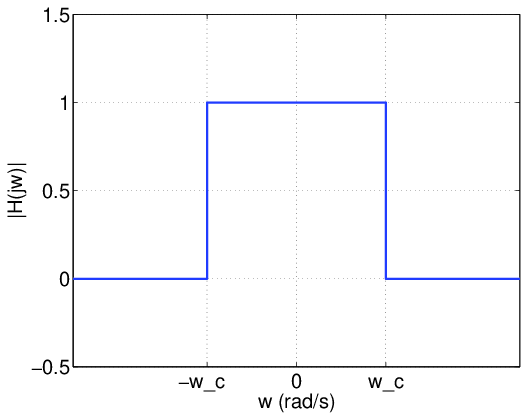
\includegraphics[width=3.2cm]{Figures/FiltroPBaja.png}
                \end{figure}
                \vspace{-0.2cm}
            }
            \visible<2->{
                \scriptsize
                \centering{Filtro paso alta}
                \vspace{0.1cm}
                $H(j\omega)\!=\!\left \{  \!\!\!\begin{array}{l} 0, \: \textrm{para } |\omega|\!\!<\!\!\omega_c\\1, \:\textrm{c.c.}  \end{array}\right .$
                \vspace{-0.4cm}
                \begin{figure}
                    \centering
                    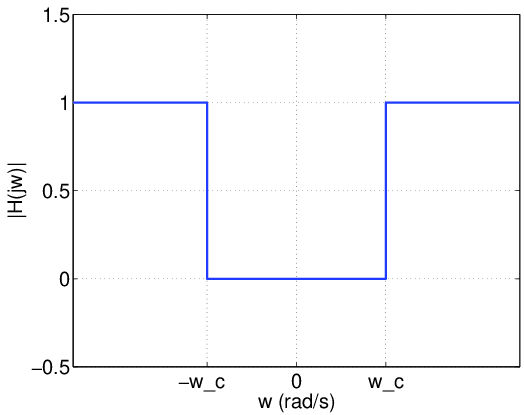
\includegraphics[width=3.2cm]{Figures/FiltroPAlta.png}
                \end{figure}
                \vspace{-0.2cm}
            }
        \end{column}
        \begin{column}{5 cm}
            \visible<3->{
                \scriptsize
                \centering{Filtro paso banda}
                \vspace{0.1cm}
                $H(j\omega)\!=\!\left \{  \!\!\!\begin{array}{l} 1, \:  \omega_{c_1}\!\!<\!\!\omega\!\!<\!\!\omega_{c_2}\\0, \:\textrm{c.c.}  \end{array}\right .$
                \vspace{-0.4cm}
                \begin{figure}
                    \centering
                    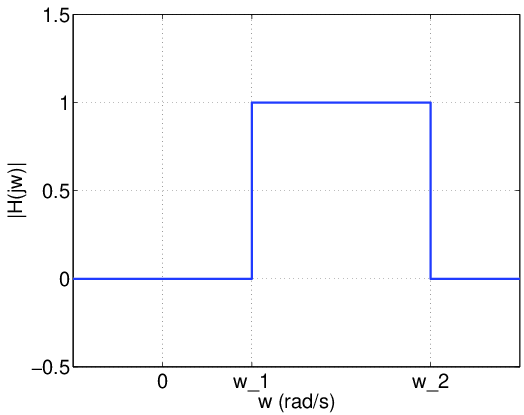
\includegraphics[width=3.2cm]{Figures/FiltroPBanda.png}
                \end{figure}
                \vspace{-0.2cm}               
            }
            \visible<4->{
                \centering{Filtro supresor banda}
                \vspace{0.1cm}
                $H(j\omega)\!=\!\left \{  \!\!\!\begin{array}{l} 0, \:  \omega_{c_1}\!\!<\!\!\omega\!\!<\!\!\omega_{c_2}\\1, \:\textrm{c.c.}  \end{array}\right .$
                \vspace{-0.4cm}
                \begin{figure}
                    \centering
                    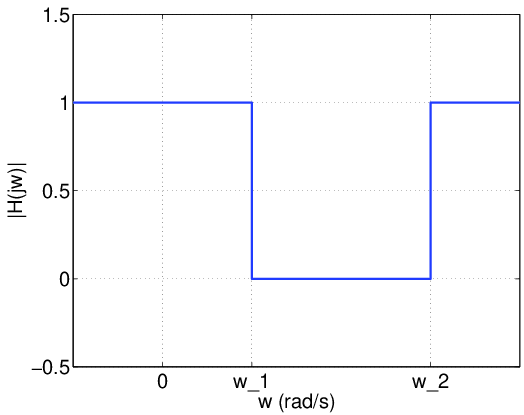
\includegraphics[width=3.2cm]{Figures/FiltroSBanda.png}
                \end{figure}
                \vspace{-0.2cm}
            }    
        \end{column}
    \end{columns}
\end{frame}
\section{Filtros Continuos}
\subsection{Filtros continuos generales}


\begin{frame}
    \frametitle{Filtros Continuos Generales I}
    \footnotesize
    El comportamiento en frecuencia de un filtro continuo queda determinado por la posici\'{o}n de los polos y los ceros de su funci\'{o}n de transferencia $H(s)$.
    \vspace{0.1cm}
    Podemos recordar, de sistemas lineales, los comportamientos que se observan al representar la respuesta en frecuencia de diferentes filtros b\'{a}sicos (sistemas estables).
    \vspace{0.1cm}

    \begin{columns}[c]
        \hspace{0.7cm}\begin{column}{6cm}
            \alert{Polo simple}: $H(s)=\frac{a}{s+a}$, (\color{olivegreen}Ej: \color{black}a=10)
            \vspace{0.1cm}
            \scriptsize
            Atenúa, pero no totalmente.
            Si usamos varios polos simples atenuará  mas rápido.
            \vspace{0.1cm}
            \begin{figure}\centering
                \includegraphics[width=5cm]{./Figures/FiltroContinuo1b.eps}
            \end{figure}
            \vspace{-0.4cm}
        \end{column}

        \begin{column}{6cm}
            \vspace{-0.0cm}
            \alert{Cero simple: }$H(s)=\frac{s+a}{a}$, (\color{olivegreen}Ej: \color{black}a=10)
            \vspace{0.2cm}\scriptsize
            Amplifica, continuamente.
            \vspace{0.1cm}
            \begin{figure}\centering
                \includegraphics[width=5cm]{./Figures/FiltroContinuo2b.eps}
            \end{figure}
        \end{column}
    \end{columns}
\end{frame}


\begin{frame}
    \frametitle{Filtros Continuos Generales II}

    \footnotesize
    \begin{columns}[c]
        \hspace{0.7cm}\begin{column}{6cm}
            \alert{Polo doble: }$H(s)=\frac{\sigma^2+\omega_a^2}{s^2+2\sigma s +\sigma^2+\omega_a^2 }$,
            \scriptsize
            \vspace{0.1cm}
            \hspace{1.6cm}(\color{olivegreen}Ej: \color{black} $\sigma=1$, $\omega_a=3$)
            \vspace{-0.1cm}
            \begin{figure}\centering
                \includegraphics[width=3.5cm]{./Figures/FiltroContinuo3b.eps}
            \end{figure}
        \end{column}
        \begin{column}{6cm}
            \alert{Cero doble: }$H(s)=\frac{s^2+2\sigma s +\sigma^2+w_a^2 }{\sigma^2+w_a^2}$,
            \scriptsize
            \vspace{0.1cm}
            \hspace{1.6cm}(\color{olivegreen}Ej: \color{black} $\sigma=1$, $w_a=3$)
            \vspace{-0.1cm}
            \visible<2->{\begin{figure} \centering \includegraphics[width=3.5cm]{./Figures/FiltroContinuo4b.eps}  \end{figure}}
        \end{column}
    \end{columns}

    \begin{columns}[c]
        \hspace{0.7cm}\begin{column}{6cm}
        \alert{Polo doble:}$H(s)=\frac{\omega_n^2}{s^2+\omega_n^2 }$,  (\color{olivegreen}Ej: \color{black} $\omega_n=3$)
        \scriptsize
        \vspace{0.1cm}
        Es inestable para $\omega=\omega_n$
        \vspace{-0.1cm}
        \begin{figure}\centering
            \includegraphics[width=3.5cm]{./Figures/FiltroContinuo5b.eps}
        \end{figure}
    \end{column}
    \vspace{0.1cm}
    \begin{column}{6cm}
        \alert{Cero doble: }$H(s)=\frac{s^2+\omega_n^2 }{\omega_n^2}$, (\color{olivegreen}Ej: \color{black}$\omega_n=3$)
        \scriptsize
        \vspace{0.1cm}
        atenua totalmente a $\omega=\omega_n$
        \vspace{-0.1cm}
        \begin{figure}\centering
            \includegraphics[width=3.5cm]{./Figures/FiltroContinuo6b.eps}
        \end{figure}
        \end{column}
    \end{columns}
\end{frame}

%%%%%%%%%%%%%%%%%%%%%%%%%%%%%


\begin{frame}
    \frametitle{Filtros Continuos Generales III}
    \footnotesize
    Para obtener la función de transferencia de un filtro continuo podemos:
    \begin{itemize}
        \item Colocar dos ceros imaginarios puros sobre las frecuencias $\omega_n$ que deseamos eliminar completamente
        \item Compensar la amplificación asociada a cada cero, con un polo con parte real negativa (eligiendo el valor de la $a$ o de la $\omega_a$ de forma apropiada).
        \item Necesitamos al menos tantos polos como ceros que el sistema sea causal (y para atenuar la amplificación continua final asociada a cada cero).
    \end{itemize}
    Sin embargo, este método no es siempre trivial (muchos parámetros).
\end{frame}


\begin{frame}
  \frametitle{Conceptos Importantes}
  \begin{itemize}
    \item \alert{¿Qué es un filtro?}
    \begin{itemize}
      \item Dispositivo que modifica selectivamente las frecuencias.
      \[
        h(t) \Leftrightarrow H(j\omega),
        \quad
        h[n] \Leftrightarrow H(\text{e}^{j\omega})
      \]
    \end{itemize}
    \item \alert{Filtros ideales}
    \begin{itemize}
      \item paso bajo,
      \item paso alto,
      \item paso banda,
      \item supresor de banda.
    \end{itemize}
    \vspace{0.2cm}

    \item \alert{¿Cómo diseñar un filtro continuo?}
    \begin{itemize}
      \item Podemos añadir ceros y polos a conveniencia.
      \item Es un método no sistemático y tedioso.
    \end{itemize}
  \end{itemize}

\end{frame}

\end{document}
